\section{Network-Informed Restoration}
\label{sec:restoration}

\subsection{Shared damage states and repair budgets}
\label{shared-damage-states-and-repair-budgets}

On the 5,000-node graph, we randomly removed 30\% or 50\% of the edges
(35,367 or 58,946 edges) while keeping all nodes intact. For each deletion
fraction $f$ and each of ten random damage orders, all four policies started
from the same damaged graph and restored 0\%, 5\%, 10\%, or 20\% of the
deleted edges. At the 5\%, 10\%, and 20\% budgets, policies restored 1,768,
3,537, and 7,073 edges after 30\% deletion, and 2,947, 5,895, and 11,789
edges after 50\% deletion, with every policy filling its budget in full.

The 200 queries were split by query ID into 140 training queries for
edge ranking and 60 held-out test queries for evaluation, ensuring that
test queries never informed policy rankings. After each repair, we measured
the giant connected component (GCC) as a fraction of the original 5,000
nodes alongside held-out retrieval success at $L=2$ and $L=3$. Before
repair, the unrepaired baselines already differed sharply across metrics:
at $f=0.30$, mean unrepaired values were $99.204 \pm 0.104\%$ for GCC,
$93.50 \pm 5.18\%$ for $L=3$, and $68.33 \pm 6.38\%$ for $L=2$; at
$f=0.50$, they were $98.218 \pm 0.128\%$ for GCC, $83.50 \pm 7.13\%$ for
$L=3$, and $42.33 \pm 4.32\%$ for $L=2$. Subtracting each seed's unrepaired
baseline from its post-repair value gives paired gains, which we summarize
as means and sample standard deviations (SD) across the ten seeds.

\subsection{Four restoration policies}
\label{four-restoration-policies}

Each policy defines a fixed ordering over deleted edges on a given damaged
graph, so larger budgets restore longer prefixes of the same ranking.
Random restoration shuffles all deleted edges uniformly and serves as an
uninformed baseline. Edge-betweenness restoration filters the intact-graph
edge-betweenness ranking to the deleted edges, prioritizing structural
bridges without using query or relation labels. Relation-type restoration
randomly orders deleted drug--protein and disease--protein edges without
substituting protein--protein interactions, isolating the effect of
restricting repairs to the relation types required by two-hop paths.

Static task-aware restoration scores deleted edges once on the initial
damaged graph using training queries that have lost all two-hop paths. Each
broken two-hop path missing exactly one edge contributes one point to that
missing edge, while paths missing both edges and already-successful
training queries contribute zero. Deleted edges are then ranked in
descending order of score, with ties---including zero-score edges---broken
randomly.

\subsection{Recovery depends on target metric, budget, and query horizon}
\label{recovery-depends-on-budget-and-query-horizon}

Figure~\ref{fig:restoration-retrieval} compares held-out retrieval gains
across both damage levels and query horizons, and
Table~\ref{tab:restoration-gains} summarizes the 20\% budget at $f=0.50$.
Across these settings, policy performance depends strongly on whether
repair targets global connectivity, short-horizon retrieval ($L=2$), or
longer-horizon retrieval ($L=3$).

\begin{table}[htbp]
  \centering
  \caption{Paired gains after restoring 20\% of the edges removed at
  $f=0.50$ (11,789 restored edges). Values are means $\pm$ sample SD in
  percentage points over ten damage seeds. Unrepaired baselines are
  $42.33 \pm 4.32\%$ ($L=2$), $83.50 \pm 7.13\%$ ($L=3$), and
  $98.218 \pm 0.128\%$ (GCC).}
  \label{tab:restoration-gains}
  \begin{tabular}{@{}lccc@{}}
    \toprule
    Policy & $L=2$ retrieval & $L=3$ retrieval & GCC fraction \\
    \midrule
    Random            & $13.17 \pm 2.77$ & $8.33 \pm 5.77$  & $0.584 \pm 0.106$ \\
    Edge betweenness  & $42.00 \pm 3.99$ & $16.50 \pm 7.13$ & $1.782 \pm 0.128$ \\
    Relation type     & $48.50 \pm 6.69$ & $15.67 \pm 7.34$ & $0.610 \pm 0.129$ \\
    Static task-aware & $24.83 \pm 6.31$ & $12.33 \pm 6.63$ & $0.670 \pm 0.085$ \\
    \bottomrule
  \end{tabular}
\end{table}

\begin{figure}[htbp]
  \centering
  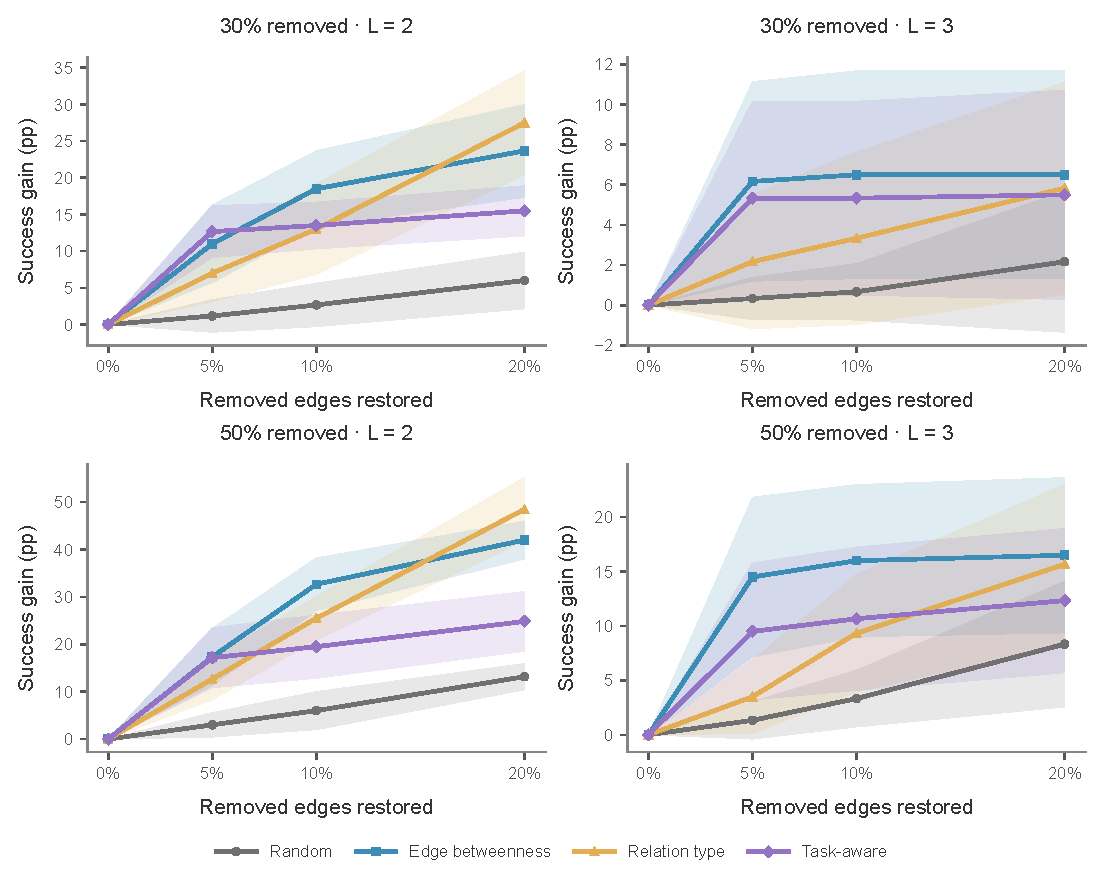
\includegraphics[width=\linewidth]{act3/final/primekg_5000_bfs_v1/fig_restoration.pdf}
  \caption{Held-out retrieval gains for the four repair policies at $L=2$ and
  $L=3$, after 30\% or 50\% edge loss. The horizontal axis gives the share of
  deleted edges restored. Lines show means of paired gains over ten damage
  seeds, and shading shows one sample SD.}
  \label{fig:restoration-retrieval}
\end{figure}

For two-hop retrieval, policy rankings cross over as the budget grows. At
30\% edge loss and a 5\% budget (1,768 edges), static task-aware repair
achieved the largest mean two-hop gain at $12.67 \pm 3.53$ percentage
points, ahead of edge betweenness ($11.00 \pm 5.28$), relation type
($7.00 \pm 3.91$), and random ($1.17 \pm 2.23$). At 50\% edge loss and a
5\% budget (2,947 edges), edge betweenness ($17.33 \pm 5.99$) and static
task-aware ($17.17 \pm 6.34$) were nearly tied at the top, ahead of
relation type ($12.67 \pm 4.39$) and random ($3.00 \pm 2.58$). Once the
budget reached 20\%, however, relation type pulled clearly ahead at both
damage levels, gaining $27.50 \pm 7.08$ points at $f=0.30$ and
$48.50 \pm 6.69$ points at $f=0.50$ (recovering 84\% of the lost two-hop
queries), compared with $23.67$ and $42.00$ points for edge betweenness and
only $15.50$ and $24.83$ points for static task-aware.

Marginal efficiency, plotted in Figure~\ref{fig:restoration-efficiency} as
paired retrieval gain per 1,000 restored edges, highlights the same
contrast between front-loaded and steady policies. At $f=0.30$ and a 5\%
budget, static task-aware delivered the highest efficiency at $7.16$
percentage points per 1,000 edges (versus $6.22$ for edge betweenness and
$3.96$ for relation type), but its efficiency fell steeply to $2.19$ points
per 1,000 edges at the 20\% budget ($5.83 \to 2.11$ at $f=0.50$).
Relation-type repair, in contrast, maintained nearly flat marginal returns
across all budgets ($3.96 \to 3.68 \to 3.89$ at $f=0.30$;
$4.30 \to 4.33 \to 4.11$ at $f=0.50$).

\begin{figure}[htbp]
  \centering
  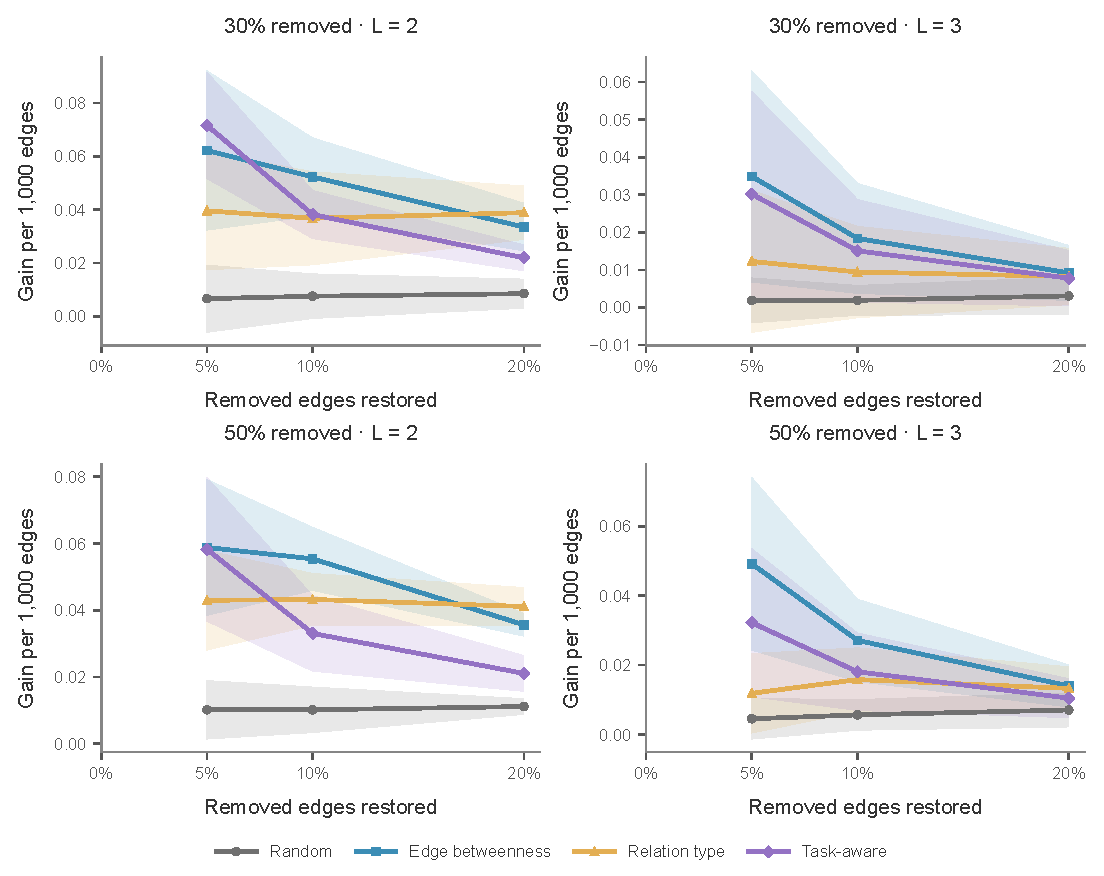
\includegraphics[width=\linewidth]{act3/final/primekg_5000_bfs_v1/fig_gain_per_edge.pdf}
  \caption{Mean gain in retrieval success fraction per 1,000 restored edges.
  For each seed, we divide the paired gain by the actual number of restored
  edges and multiply by 1,000 before averaging. Shading shows one sample SD
  across ten seeds. Efficiency is defined only for positive repair budgets.}
  \label{fig:restoration-efficiency}
\end{figure}

Global connectivity and longer-horizon retrieval instead favored edge
betweenness and reached their ceilings early. At 50\% edge loss, edge
betweenness increased the GCC fraction by $1.782 \pm 0.128$ points already
at the 10\% budget---completely restoring 100\% GCC connectivity---whereas
random ($0.584$), relation type ($0.610$), and static task-aware ($0.670$)
remained below $0.7$ points even at the 20\% budget
(Table~\ref{tab:restoration-gains} and Figure~\ref{fig:restoration-gcc}).
The same full GCC recovery occurred by the 10\% budget at $f=0.30$
($+0.796$ points). At $L=3$, the unrepaired baseline is already high
($93.50\%$ at $f=0.30$ and $83.50\%$ at $f=0.50$), leaving less headroom.
Edge betweenness closed the entire $L=3$ gap ($+6.50$ points by the 10\%
budget at $f=0.30$; $+16.50$ points at the 20\% budget at $f=0.50$), while
relation type reached $+15.67$ points at $f=0.50$, leaving only a narrow
$0.83$-point margin right against the 100\% ceiling. Thus, the policy that
maximized structural recovery differed from the policy that maximized
large-budget two-hop retrieval.

\begin{figure}[htbp]
  \centering
  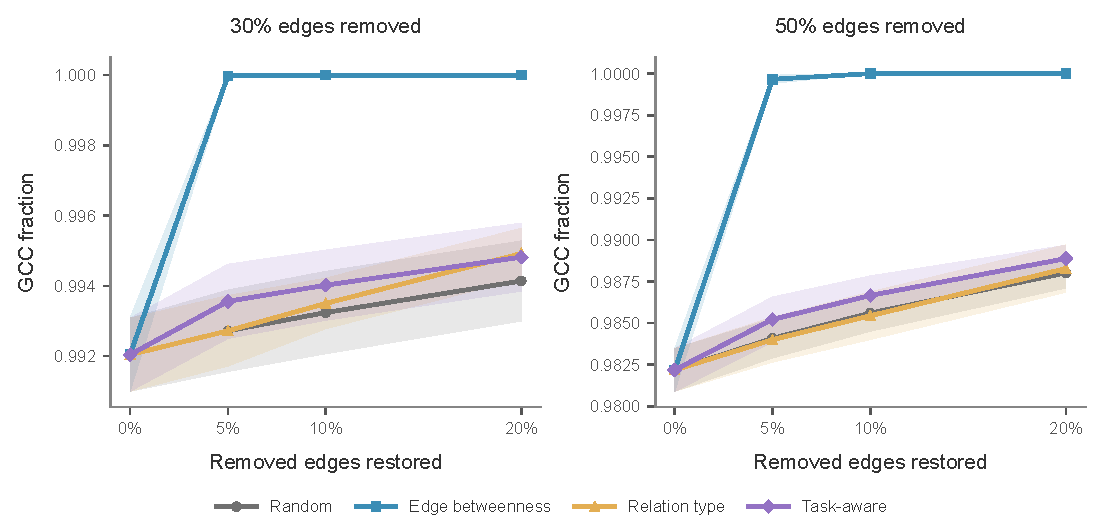
\includegraphics[width=\linewidth]{act3/final/primekg_5000_bfs_v1/fig_restoration_gcc.pdf}
  \caption{GCC fraction after repair at 30\% and 50\% initial edge loss.
  Values are fractions of the original 5,000 nodes. Lines show means and
  shading shows one sample SD over the ten damage seeds.}
  \label{fig:restoration-gcc}
\end{figure}

\subsection{Why the policies diverge: score saturation and edge-type mix}
\label{interpreting-the-static-score}

Two diagnostics explain both the budget crossover and the gap between
structural and functional recovery. First, the static task-aware score
saturates almost immediately. Across the ten damage seeds, only 31--46
deleted edges had positive static scores at 30\% deletion and 62--87 at 50\%
deletion. Those edges accounted for at most $2.6\%$ (at $f=0.30$) and
$3.0\%$ (at $f=0.50$) of the 5\% budget, and less than $0.8\%$ of the 20\%
budget. After restoring that small set of high-impact edges---which drives
its strong 5\%-budget jump---the policy spends more than 97\% of the budget
on randomly ordered zero-score edges, effectively behaving like random
repair thereafter.

Second, Figure~\ref{fig:restoration-composition} shows how each policy
allocated its budget across relation types. In the intact 5,000-node graph,
protein--protein interactions make up 76.5\% of all edges, disease--protein
relations 23.1\%, and drug--protein relations only 0.40\%. At 50\% edge loss
and a 20\% budget, static task-aware repair spent 76.0\% of its budget on
protein--protein edges (matching random's 76.4\% once zero-score ties
dominate), and edge betweenness spent 68.1\% on protein--protein edges.
Relation-type repair instead spent 100\% of its budget on the terminal
relations required by two-hop paths (98.3\% disease--protein and 1.7\%
drug--protein), explaining its sustained $L=2$ gains at larger budgets.

\begin{figure}[H]
  \centering
  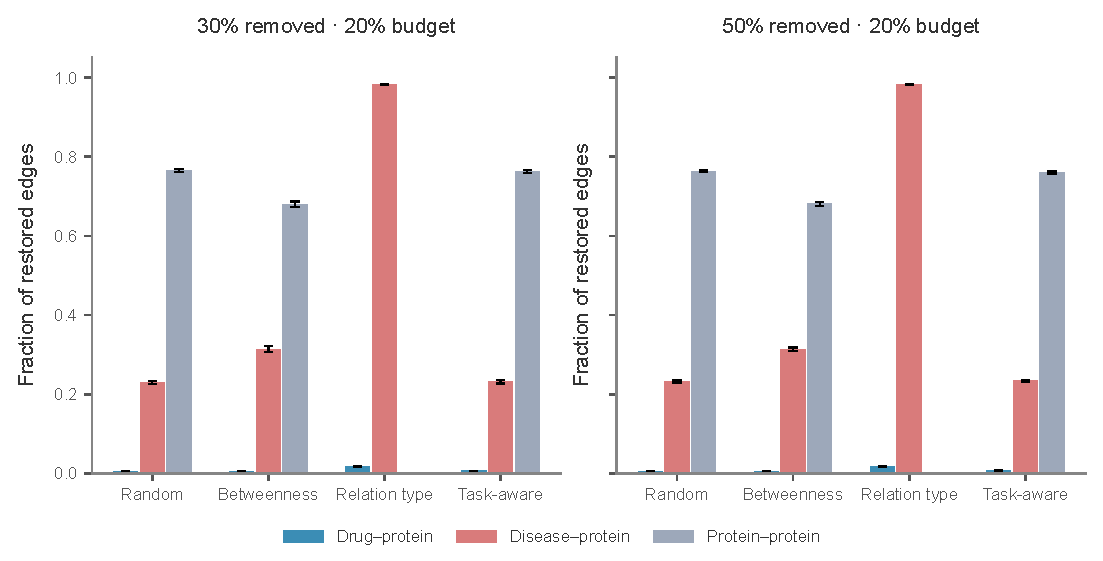
\includegraphics[width=0.9\linewidth]{act3/final/primekg_5000_bfs_v1/fig_restored_edge_types.pdf}
  \caption{Relation types among the edges actually restored with a 20\% repair
  budget. Bars show the mean share of each relation type. Error bars show one
  sample SD over ten damage seeds.}
  \label{fig:restoration-composition}
\end{figure}

Edge-type allocation also clarifies why edge betweenness performed much
better on $L=2$ than random repair despite ignoring relation labels. Because
drugs have much lower mean degree than proteins or diseases
(Section~\ref{sec:data}), deleted drug--protein edges often act as
high-betweenness bridges: at the 5\% budget, drug--protein edges made up
$1.31$--$1.34\%$ of edge-betweenness repairs, more than three times their
$0.42$--$0.44\%$ share under random repair. At the same time, its large
allocation to high-betweenness protein--protein bridges explains why it
dominated GCC and $L=3$ recovery, where a single protein--protein step can
reconnect many failed queries.

These results also point to clear directions for refinement. Because the
140/60 split is defined over query IDs, training and test queries can share
drug or disease endpoints, and the static score is computed once from
two-hop training paths without updating as edges are restored or adapting
to three-hop paths. Extending the scoring rule to update iteratively or to
incorporate longer paths would test how much further task-aware restoration
can go once score saturation is removed.
